%\documentclass[letterpaper,12pt]{article}
\documentclass[12pt]{book}

% page dimensions
\newcommand{\cardHeight}{4.25}
\newcommand{\cardWidth}{5.5}
\newcommand{\halfHeight}{2.125}
\newcommand{\halfWidth}{2.75}

% --- Packages
\usepackage[paperwidth= \cardWidth in, paperheight=\cardHeight in,top=0in, bottom=0in, left=0in, right=0in]{geometry}
%\usepackage[landscape]{geometry}

\usepackage{tikz} 			%draw

\usepackage{fontspec}		%Set font
\setmainfont{Orbit}         % special by Evan Pittson Design

\usepackage{ifthen}			% if then else



% --- Formatting
\pagenumbering{gobble}
\setlength{\parindent}{0pt}


% --- Defined Values
% Constants
\newcommand{\altMargin}{1}
%\newcommand{\cardHeight}{4.25}
%\newcommand{\cardWidth}{5.5}
\newcommand{\lrMarginStart}{2.7}
\newcommand{\udMarginStart}{2.2}
\newcommand{\senderNAnchor}{1.7}
\newcommand{\recipientSAnchor}{-1.9}
\newcommand{\sender}{Sender}
\newcommand{\recipient}{Recipient}

% Set Specific Variables
\newcommand{\setNumberStart}{0}
\newcommand{\setNumberEnd}{5}
\newcommand{\setNumberIncrement}{1}
\newcommand{\cardNumberStart}{1}
\newcommand{\cardNumberEnd}{5}
\newcommand{\cardNumberIncrement}{1}
\newcommand{\setNumber}{0}
%\newcommand{\cardNumber}{1}
\newcommand{\cardTitle}{title goes here}
\newcommand{\senderOn}{0}
\newcommand{\recipientOn}{0}
%\newcommand{\qrkNumber}{QRK$\;$M$7_{\setNumber}\;20200530:\cardNumber/20\smile\setNumber/20\;$T$9$ }





% Styling
\newcommand{ \cardTitleSty }[1]{\raggedright \large \MakeUppercase #1}
\newcommand{ \personSty }[1]{\raggedright \normalsize \MakeUppercase #1}
% Instructions
\newcommand{\single}[1]{#1}							
\newcommand{\double}[2]{#1,#2}
\newcommand{\triple}[3]{#1,#2,3}
\newcommand{\singleSingle}[2]{#1,#2}
\newcommand{\doubleSingle}[3]{#1,#2,#3}
\newcommand{\tripleSingle}[4]{#1,#2,#3,#4}
\newcommand{\singleDouble}[3]{#1,#2,#3}
\newcommand{\doubleDouble}[4]{#1,#2,#3,#4}
\newcommand{\tripleDouble}[5]{#1,#2,#3,#4,#5}
\newcommand{\singleTriple}[4]{#1,#2,#3,#4}
\newcommand{\doubleTriple}[5]{#1,#2,#3,#4,#5}
\newcommand{\tripleTriple}[6]{#1,#2,#3,#4,#5,#6}



\begin{document}

	\foreach \card in {\cardNumberStart,...,\cardNumberEnd}
	{	
		%\newcommand{\cardNumber}{\card}
		\begin{center}
			\begin{figure}
				\resizebox{\paperwidth}{\paperheight}
				{ %Generate QRK Number
\newcommand{\qrkNumber}{QRK$\;$M$7_{\iterationNumber}\;20200530:\card/20\smile\set/20\;$T$9$ }
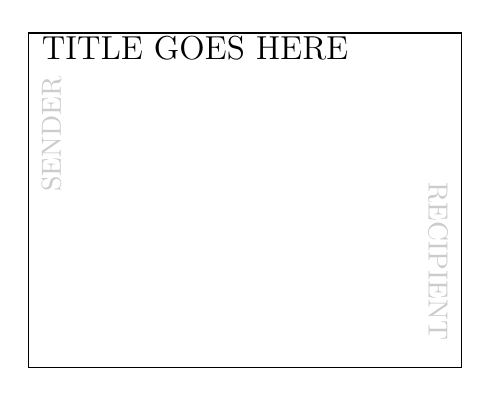
\begin{tikzpicture}[]	
		% card
    	\draw (-\halfWidth,-\halfHeight) rectangle (\halfWidth,\halfHeight);
    	
    	% title
    	\node[anchor=north west] at (-\lrMarginStart,\udMarginStart) { \cardTitleSty{\cardTitle}};
    	
    	% QRK Number
    	\node[anchor=south west] at (-\lrMarginStart, -\udMarginStart) { \tiny \qrkNumber};

    	% sender label 
    	\ifthenelse{\senderOn = 1}
    					 % for the sender
    					 {\node[anchor=north east, rotate = 90] at (-\lrMarginStart,\senderNAnchor) {\personSty{\sender}};}
    					 % not for sender
    					 {\node[anchor=north east, rotate = 90, text = black!20!white] at (-\lrMarginStart,\senderNAnchor) {\personSty{\sender}};} 

    	% recipient label 
    	\ifthenelse{\recipientOn = 1}
    					 % for the recipient
    					 {\node[anchor=north east, rotate = -90 ] at (\lrMarginStart, \recipientSAnchor) {\personSty{\recipient}};}
    					 % not for recipient
    					 {\node[anchor=north east, rotate = -90, text = black!20!white ] at (\lrMarginStart,\recipientSAnchor) {\personSty{\recipient}};} 
    					 
    	% instructions
    	\node[anchor = north west] at (-1.5, 0.9) { \instructionFormatting{\tripleOne} } ;
    	\node[anchor = north west] at (-1.5, 0.4) {\instructionFormatting{\tripleTwo}} ;
    	\node[anchor = north west] at (-1.5, -0.1) {\instructionFormatting{\tripleThree}} ;		
\end{tikzpicture}}
			\end{figure}
		\end{center}
	}
	
\end{document}